%!TeX spellcheck = en-US,en-DE
\documentclass[a4paper,11pt]{report}


%%%%%%%%%%%%%%%%%%%%%%%%%%%%
% University of Sussex thesis template
%%%%%%%%%%%%%%%%%%%%%%%%%%%%
% Modification History
%
% Based on usthesis.cls by Jonathon Read
% http://www.cogs.susx.ac.uk/users/jlr24/latex.html
% Modified by Anthony Smith, Feb 2007
% Incorporated into single thesis.tex file, Anthony Smith, 30 June 2008
% Minor alterations to page numbering, AJS, 25 July 2008
% New alternative hyperref options for print version, AJS, 11 Sep 2008
% "DRAFT" on header, AJS, 12 Sep 2008
%%%%%%%%%%%%%%%%%%%%%%%%%%%%


%%%%%%%%%%%%%%%%%%%%%%%%%%%%
% LINE SPACING
\newcommand{\linespacing}{1.5}
\renewcommand{\baselinestretch}{\linespacing}
%%%%%%%%%%%%%%%%%%%%%%%%%%%%


%%%%%%%%%%%%%%%%%%%%%%%%%%%%
% BIBLIOGRAPHY STYLE
\usepackage{natbib}
% \bibliographystyle{plain} for [1], [2] etc.
\bibliographystyle{apalike}
%%%%%%%%%%%%%%%%%%%%%%%%%%%%


%%%%%%%%%%%%%%%%%%%%%%%%%%%%
% OTHER FORMATTING/LAYOUT DECLARATIONS
% Graphics
\usepackage{graphicx,color}
\usepackage{csquotes}
\usepackage{epstopdf}
\usepackage[british]{babel}
% The left-hand-side should be 40mm.  The top and bottom margins should be
% 25mm deep.  The right hand margin should be 20mm.
\usepackage[a4paper,top=2.5cm,bottom=2.5cm,left=4cm,right=2cm,headsep=10pt]{geometry}
\flushbottom
% Pages should be numbered consecutively thorugh the main text.  Page numbers
% should be located centrally at the top of the page.
\usepackage{fancyhdr}
\fancypagestyle{plain}{
	\fancyhf{}
	% Add "DRAFT: <today's date>" to header (comment out the following to remove)
	%\lhead{\textit{DRAFT: \today}}
	%
	\chead{\thepage}
	\renewcommand{\headrulewidth}{0pt}
}
\pagestyle{plain}
%%%%%%%%%%%%%%%%%%%%%%%%%%%%


%%%%%%%%%%%%%%%%%%%%%%%%%%%%
% ANY OTHER DECLARATIONS HERE:

%%%%%%%%%%%%%%%%%%%%%%%%%%%%


%%%%%%%%%%%%%%%%%%%%%%%%%%%%
% HYPERREF
\usepackage[colorlinks,pagebackref,pdfusetitle,urlcolor=blue,citecolor=blue,linkcolor=blue,bookmarksnumbered,plainpages=false]{hyperref}
% For print version, use this instead:
%\usepackage[pdfusetitle,bookmarksnumbered,plainpages=false]{hyperref}
%\usepackage{backref}
%\renewcommand{\backrefpagesname}{Cited on}
%%%%%%%%%%%%%%%%%%%%%%%%%%%%


%%%%%%%%%%%%%%%%%%%%%%%%%%%%
% BEGIN DOCUMENT
\begin{document}
%%%%%%%%%%%%%%%%%%%%%%%%%%%%


%%%%%%%%%%%%%%%%%%%%%%%%%%%%
% PREAMBLE: roman page numbering i, ii, iii, ...
\pagenumbering{roman}
%%%%%%%%%%%%%%%%%%%%%%%%%%%%


%%%%%%%%%%%%%%%%%%%%%%%%%%%%
%% TITLE PAGE: The title page should give the following information:
%%	(i) the full title of the thesis and the sub-title if any;
%%	(ii) the full name of the author;
%%	(iii) the qualification aimed for;
%%	(iv) the name of the University of Sussex;
%%	(v) the month and year of submission.
\thispagestyle{empty}
\begin{flushright}

\includegraphics[width=6cm]{uslogo}
\end{flushright}
\vskip40mm
\begin{center}
% TITLE
\huge\textbf{Predicting share prices using natural language engineering and machine learning techniques.}
\vskip2mm
% SUBTITLE (optional)
% \LARGE\textit{How it all works}
\vskip5mm
% AUTHOR
% \Large\textbf{Samuel Johnson}
\normalsize
\end{center}
\vfill
\begin{flushleft}
\large
% QUALIFICATION
University of Sussex	\\
% DATE OF SUBMISSION
May	 2018
\end{flushleft}
%%%%%%%%%%%%%%%%%%%%%%%%%%%%


%%%%%%%%%%%%%%%%%%%%%%%%%%%%
% DECLARATIONS
\chapter*{Declaration}
This report is submitted as part requirement for the degree of Computer Science at the University of Sussex. It is the product of my own labour except where indicated in the text. The report may be freely copied and distributed provided the source is acknowledged.

% ADDITIONAL DECLARATIONS HERE (IF ANY)

\vskip5mm
Signature:
\vskip20mm
% AUTHOR
Samuel Johnson
%%%%%%%%%%%%%%%%%%%%%%%%%%%%

%%%%%%%%%%%%%%%%%%%%%%%%%%%%
% ACKNOWLEDGEMENTS
\chapter*{Acknowledgements}
\renewcommand{\baselinestretch}{\linespacing}
\small\normalsize
% ACKNOWLEDGEMENTS HERE:
Bill Keller\\
Dad\\
Mum\\
Robert\\
Emily\\
%%%%%%%%%%%%%%%%%%%%%%%%%%%%

%%%%%%%%%%%%%%%%%%%%%%%%%%%%
% SUMMARY PAGE
\thispagestyle{empty}
\newpage
\null\vskip10mm
\begin{center}
\large
\underline{UNIVERSITY OF SUSSEX}
\vskip20mm
% AUTHOR, QUALIFICATION
\textsc{Samuel Johnson}
\vskip20mm
% TITLE
\underline{\textsc{Predicting share prices using natural language engineering and machine learning techniques}}
\vskip0mm
% SUBTITLE (optional)
% \underline{\textsc{How it all works}}
\vskip20mm
\underline{\textsc{Summary}}
\vskip2mm
\end{center}
% Change line spacing
\renewcommand{\baselinestretch}{1.0}
\small\normalsize
% SUMMARY HERE (300 word limit for most subjects):

%%%%%%%%%%%%%%%%%%%%%%%%%%%%




%%%%%%%%%%%%%%%%%%%%%%%%%%%%
% TABLE OF CONTENTS, LISTS OF TABLES & FIGURES
\newpage
\pdfbookmark[0]{Contents}{contents_bookmark}
\tableofcontents
\listoftables
\phantomsection
\addcontentsline{toc}{chapter}{List of Tables}
\listoffigures
\phantomsection
\addcontentsline{toc}{chapter}{List of Figures}
%%%%%%%%%%%%%%%%%%%%%%%%%%%%


%%%%%%%%%%%%%%%%%%%%%%%%%%%%
% MAIN THESIS TEXT: arabic page numbering 1, 2, 3, ...
\newpage
\pagenumbering{arabic}
%%%%%%%%%%%%%%%%%%%%%%%%%%%%


%-----------------------------------------------------
% Chapter: Introduction
%-----------------------------------------------------
\chapter{Introduction}
\label{chap:intro}

Data mining and natural language processing are some of the fastest growing fields in computer science. This is a result of many factors, the most notable being the emergence of the World Wide Web.  Consequently, millions of interconnected documents can be viewed and shared by 3.2 billion people. This continuous stream of information provides one of the largest and diverse data sets to mine and harvest information from. Another factor is the investment that commercial companies are making to see how they can exploit large data sets to use the information to their advantage. An example of this is mining and extracting customer opinions about a given product found on the web. Using this information could lead to improvements in a company's product and also give a better understanding of their customer's needs.

The financial sector is one example of where significant investment is being made. Brokerage firms and investors are spending their time and money harvesting a range of data with the aim that the data will give them an informational advantage when trading shares. The type of data collected can range from statistical financial data to textual information from the web. Financial data is used to help make forecast behaviour based on historical data. To find these patterns, statistical analysis or simulations can be used. Textual information can be useful to discover consumer trends and opinions. One method to achieve this is through scraping HTML documents from microblog sites such as Twitter. This is useful for brokers: to consumer opinions may hint at the future performance of a given stock. Another reason behind the interest in both these fields is the speed at which computers can analyse data. On average, adults read 250-300 words per minute whereas a computer can download and analyse data at speed magnitudes faster. This processing power can provide real informational advantages when making decisions on investments.

One possible dataset that could be used by brokers to give an indication of stock performance is digital news articles. Major news organisations such as "The New York Times" and "The Wall Street Journal" release on average over 200 stories and videos a day. Most of this content contains well written factual information and presents knowledgeable opinions. While there has been research on using financial based news stories, there has not been many studies that have investigated the value of other categorised articles. This lack of knowledge inspires research and development into testing the following hypothesis:\\

\noindent\fbox{%
    \parbox{\textwidth}{%
        \textbf{Hypothesis:}\\
        The sentiment of news articles produced by mainstream news based on a given company correlates with the performance of that given company's share value.
    }%
}

\clearpage

To test this hypothesis, this experiment will be focusing on following the value of two highly valued companies, Apple and Facebook. This is due to them having a large media presence and having articles written about them on a regular basis. Alongside this, articles that are written about technology and other technology companies will be collected. This is to see if a correlation can be found between the general sentiment of the technology sector and the markets' value.

The experiment has two main phases, the first being performing sentiment analysis on newly scraped articles. The second is using statistical analysis to mark whether a given positive or negative sentiment correlates with a shares' value. Alongside the experiment, a web platform has also been produced to display the predictions made by the sentiment analysis stage. For definitions of terms, the reader is encouraged to refer tot he Nomanclature which can be found in the appendix.

%-----------------------------------------------------
% Chapter: Ethical Considerations
%-----------------------------------------------------
\chapter{Ethical considerations}
\label{chap:ethical-con}
The British Computer Society (BCS) is a respected organisation and body that represents the sector of information technology and those who work in it. They provide a set of rules and a code of conduct which it expects their members to follow. While I am not a member of this society, the rules and codes they provide are great references and points to allow me to review what I may need to consider in my project. This section of the report will explore the parts of the code of conduct are relevant to this project. Further, there are some other ethical considerations that will need to be discussed.

\section{BCS Code of conduct}

\subsection{Public interest}
Few parts of the public interest section of the code of conduct are relevant to this project. It is important to note that this project poses no physical danger to the public or myself. However, it does need to be disclosed that the system created for this experiment should not be taken as financial advice.

\subsection{Professional competence and integrity}
This section of the code of conduct is broad and focuses on my behaviour as a programmer rather than the work produced. It can be confirmed that the work undertaken is within the limits of my professional competence. Alongside this, my professional knowledge, skills and competence will be developed on a continuing basis throughout this project. It is also important to note that I am committed to respect and value alternative viewpoints when related to my work and seek criticism in order to improve myself as a programmer and the project itself. It also must be noted that I will not be susceptible to bribes or unethical inducement as stated in the conduct.

\subsection{Duty to relevant authority}
My immediate authority in the context of this project is the University of Sussex and the department of informatics. Regarding point 3B of the code of conduct, I will be strictly following the universities assessment and exam regulations. It is without question that I will avoid any situation that may give rise to a conflict of interest between me and the university and will declare any third party work that may have taken place.

\section{Other ethical considerations}
One other ethical consideration that needs to be discussed is related to web scraping. There are no specific laws that prevent me from consuming publicly available information. However, it should be noted that the owners of these articles, which in this case would be the news organisations, can claim against me if I infringe the organisations' rights or if I breach the terms and conditions of the site. I will need to keep this in mind when compiling my list of sources and respect the rights of these organisations and only use sites which allow me to scrape their articles. I will not be publishing and displaying the contents of the articles that I have scraped to avoid breaking copyright laws.

%-----------------------------------------------------
% Chapter: Background
%-----------------------------------------------------
\chapter{Background}
\label{chap:background}

In this section, the abstract problem of sentiment analysis, techniques that are used to perform sentiment analysis and a refinement of the sentiment analyis task that will be undertaken in this experiment will be discussed alongside existing studies that relate to this project.

\subsection{The abstract problem of sentiment anaylsis}
Before advancing, it is sensible to discuss what the task of sentiment analysis involves in further detail. Bing Lui describes the problem of sentiment analysis as:

\begin{displayquote}
Sentiment analysis, also called opinion mining, is the field of study that analyses people’s opinions, sentiments, evaluations, appraisals, attitudes, and emotions towards entities such as products, services, organizations, individuals, issues, events, topics, and their attributes.
\end{displayquote}

To further this explanation, the definition of an opinion can be defined as the following quintuple:

\\\[Opinion (e_i, a_i_j, s_i_j_k_l, h_k, t_l)\]

In table \ref{table:sentiment}, an explanation has been provided to each component with an example related to this experiment.

\begin{table}[h!]
\centering
\caption{Abstraction of an opinion}
\label{table:sentiment}
\begin{tabular}{|l|l|}
\hline
\[e_i\] & \begin{tabular}[c]{@{}l@{}}\(e_i\) is the entity that the news article is focusing on whether it is Apple, \\Facebook or the the subject of technology.\end{tabular} \\ \hline
\[a_i_j\] & \begin{tabular}[c]{@{}l@{}}\(a_i_j\) refers to the aspect of \(e_i\). Aspect refers to a particular part \\ or feature of the entity e.g. an article about the management \\ at the company Apple would translate to Apple being the entity \\ and the management being the aspect the article is referring to.\end{tabular} \\ \hline
\[s_i_j_k_l\] & \begin{tabular}[c]{@{}l@{}}\(s_i_j_k_l\) refers to the sentiment of this aspect. In the context of this \\ project, it will output a positive or negative sentiment.\end{tabular} \\ \hline
\[h_k\] & \begin{tabular}[c]{@{}l@{}}\(h_k\) is the opinion holder, in the context of this project, it is referring \\ to the news organisation that the article has been scraped the article from.\end{tabular} \\ \hline
\[t_l\] & \begin{tabular}[c]{@{}l@{}}\(t_l\) is the time frame of the opinion. Opinions can change rapidly, \\ especially in the stock market. It will be important to get the \\ latest opinions rather than scraping older opinions that are no longer \\ relevant.\end{tabular} \\ \hline
\end{tabular}
\end{table}

\subsection{Sentiment analysis techniques}

The techniques that are used to perform sentiment analysis can be split into two categories: machine learning techniques and lexicon based techniques.

\subsubsection{Machine learning based techniques}
Machine learning based techniques refer to using machine learning algorithms such as a Naive Bayes classifier to output a classification. Most machine learning techniques are supervised based which means they require a training set. A training set is used by a  classifier to learn the differentiating characteristics of documents so that when a new article needs to be classified, it will use the previous information to return a predicted sentiment.

\subsubsection{Lexicon based techniques}
Lexicon based techniques refer to the unsupervised technique of classification. This approach involves calculating orientation for a document from the semantic orientation of words or phrases in the document. Sentiment lexicon contains lists of words and expressions used to express people’s subjective feelings and opinions. For example, start with positive and negative word lexicons, analyse the document for which sentiment need to find. Then if the document has more positive word lexicons, it is positive, otherwise, it is negative. The lexicon based techniques are unsupervised because they do not require prior training in order to classify the data.

\subsubsection{Comparison of techniques}
S.M. Vohra and J.B. Teraiya published research which compared these two techniques. They concluded that supervised machine learning techniques have shown relatively better performance than the unsupervised lexicon based methods. Yet, it is important to highlight that Vohra and Teraiya argued that unsupervised methods are still valuable because supervised methods demand large amounts of labelled training data that are very expensive to create whereas acquisition of unlabelled data is easy.

\subsection{Refining the sentiment analysis task ahead}
Now the problem of sentiment anaylsis and the techniques used to perform this task have been explained, it is suitable to formalise and refine what will be done within this experiment.

In this experiment, document sentiment anaylsis will be performed. This means the whole article will be considered as a basic information unit. Bing Lui formalises the task of document sentiment analyis as the following:

\begin{displayquote}
	Given an opinion document d evaluating an entity, determine the overall sentiment s of the opinion holder about the entity, i.e., determine s expressed on aspect GENERAL in the quintuple
	\\\[(\_, GENERAL, s,\_, \_)\]

	where the entity e, opinion holder h, and time of opinion t are assumed known or irrelevant.
\end{displayquote}

In the context of this experiment, document sentiment analysis will be used to classify whether opinions found in digital articles are positive or negative towards the entities Apple or Facebook. To perform the task of sentiment analysis, this experiment will use a range of supervised machine learning algorithms to classify news articles into positive and negative classifications.

\subsection{Existing studies}
As mentioned, sentiment analysis is a large and growing field. Previous work particularly relevant to our task falls naturally in two groups. The first relates to using sentiment analysis to find a monetary correlation. The second relates to systems that analyse sentiment on news articles.

\subsubsection{Sentiment analysis to find a monetary correlation}

Sadikov, Parameswaran and Venetis published research on using the information found on blogs as predictors of movie success. In their study, they used a pre-existing dataset to find key features of movie references in blogs and were able to identify the most useful features for making movie sale predictions. They found a low correlation between information found in blogs for the first-week movie sales but subsequent weeks are more predictive using the same information.

Bar-Haim and Feldman attempted to identify expert investors and collect the content of their microblogs where expert knowledge would be shared. The aim of scraping these blogs was to see if better predictions of the value of a company could be made. Until then, they had been using a noisy dataset which contained both poor and expert knowledge. The results concluded that using the expert opinions did cause a rise in accuracy in judging a company's value.

\subsubsection{Sentiment analysis on news articles}

Godbole, Srinivasaiah and Skiena published research based on a system that they created that assigns scores indicating positive or negative opinion for each entity in a text corpus. They then went on to analyse their system on a large corpus of news and blogs. They demonstrated through their analysis that they could identify positive entities within news articles and blogs and negative entities.

More recently, there has been research papers published based on the same idea of using sentiment analysis on news articles to identify market behaviour. Written by Joshi Kalyani, H. N. Bharathi and Rao Jyothi, the basis of their experiment was collecting years of financial news articles focused on the company Apple. Using these articles they investigated the correlation between the sentiment held towards Apple and the value of their stock. This is similar to what this study is set out to do. But, more general news articles focused on Apple and Facebook will be scraped rather than focusing on financial news.

%-----------------------------------------------------
% Chapter: Requirement Analysis
%-----------------------------------------------------
\chapter{Requirement analysis}
\label{chap:requirement-anal}

The requirement analysis stage of a project is important. It presents clear achievable goals and reduces the risk of not delivering during the design and implementation of the project. Within this chapter, both functional and nonfunctional requirements will be defined for both the research stage and the application stage. The research stage is the implementation of the pipeline that would test the hypothesis of the experiment. The application stage takes the form of a web platform that is designed to illustrate the pipeline's predictions.

\section{Functional requirements}

Functional requirements refer to what the product should be able to do and what functionality it should provide

\subsection {Research requirements}
\begin{itemize}
		\item \textbf{Implement methods to scrape HTML files found on the internet}. The base of the experiment requires digital articles to be downloaded from their sources.
		\item \textbf{Implement methods to parse through each HTML file that has been downloaded and extract their textual data.} The value of these HTML files is the articles within them. It is important to only extract the useful data for analysis rather than everything found in the file.
    \item \textbf{Preprocess each parsed HTML file into a machine readable format.} When performing NLP tasks, it is normal to preprocess textual information to standardise the data and also turn it into a format that can be analysed by algorithms.
    \item \textbf{Implement a topic classifier to classify whether an article is talking about Apple, Facebook or the Technology Sector}. It is essential that we classify newly scraped articles into a category so we can accurately track the behaviour of these companies' or sectors shares.
    \item \textbf{Implement multiple machine learning models to extract a sentiment from a preprocessed article}. These models should take as input preprocessed news articles and return the sentiment of an article (positive or negative).
    \item \textbf{Automate analysis of the sentiments collected from the HTML documents when compared against the value of shares}.
\end{itemize}

\subsection {Application requirements}
\begin{itemize}
  \item \textbf{Create a platform which displays the share behaviour predictions created by the research stage}. This is the main function of the application and will be used to demonstrate the progress and results of my experiment.
    \item \textbf{Create a platform which illustrates the behaviour of the Apple, Facebook and Technology share prices}. This will provide a graphical representation of how these companies' shares are behaving and will ease in the understanding of the context of each prediction.
    \item \textbf{Create a platform that allows users to test each machine learning model developed in the research stage in classifying sentiment}. This is another important feature of the application and will be used to demonstrate how each machine learning model behaves.
\end{itemize}

\section{Nonfunctional requirements}
Nonfunctional requirements refer to how a system should behave and how the functional requirements should be implemented.

\subsection{Research requirements}
\begin{itemize}
    \item \textbf{Scrape HTML page at a regular time interval}. This is required due to the results of this experiment being time-sensitive and requiring any new articles not to be missed.
  \item \textbf{The pipeline should be able to handle a lot of articles at once}. Alongside scraping at regular time intervals, it is important that the system can handle a large number of articles at a time as there may be an influx of news released at one point in time.
    \item \textbf{Have new articles scraped and analysed at a fast speed}. As mentioned, the results of these experiments are time-sensitive so it is important to have these analysed at a fast speed to improve accuracy when pinpointing a change in share behaviour.
    \item \textbf{Track the behaviour of Facebook / Apple / Technology value of a series of time intervals to be able to track changes across it all}. Part of this experiment is seeing how over a series of different time scales that news articles may be affecting the price of shares so it's important to implement this to get good, useful results.
\end{itemize}

\subsection{Application requirements}
\begin{itemize}
    \item \textbf{The platform should be responsive in design}. This is not essential but is an expected behaviour of modern websites created now.
    \item \textbf{The platform should have an interface which can be easily used by users}. When the platform is used, it should not create confusion and avoid frustration.
\end{itemize}

%-----------------------------------------------------
% Chapter: Project Plan
%-----------------------------------------------------
\chapter{Project Plan}
As mentioned previously, this project has two distinct parts. A research section where the hypothesis given within the introduction will be tested and an application section where a web platform will be created to display the results of the experiment. Due to these two parts contrasting, it is important to discuss both separately. At the end of this chapter, a section has been included which explains practices that will be followed in both parts.

\section{Research}
The research stage was the core of the dissertation and therefore it was sensible to predict that this was going to take the majority of the time. After research, planning and a series of discussions with Bill, my supervisor, a blueprint of the experiment was created. This blueprint took the form of a set of stages which can be seen below.

\begin{itemize}
    \item{Scan and download new articles found on news sites}
    \item{Preprocess these new articles ready for classification}
    \item{Classify the topic of a preprocessed article into Facebook, Apple or Technology categories}
    \item{Create and train a set of supervised machine learning algorithms to classify new articles}
    \item{Run sentiment analysis for each new article using each machine learning model and store their predictions}
    \item{Evaluate the recorded sentiment versus the behaviour of the price of shares}
\end{itemize}

By breaking up this section into a series of components, it allowed better planning and time management. When meeting weekly with Bill clear deliverables were organised for the next meeting for each section. It also led to the decision of using the 'event-driven programming' methodology for the majority of this section due to it being evident that there are dependencies for each task from the previous task.

\section{Application}
The application stage came second in priority for this project. This was due to the website content and requirements being heavily dependent on the experiment to be started. Just like the research stage, however, it was split into different sections. The main tasks included:

\begin{itemize}
    \item{Create a web server and environment}
    \item{Create backbone of web platform including pages and navigation}
    \item{Create a backend system to retrieve prediction data from storage}
    \item{Create tables and charts illustrating predictions made by the research stage using HTML and Javascript}
    \item{Create a system to allow users to test machine learning algorithms created in research stage}
    \item{Implement AJAX requests that can communicate with machine learning algorithms}
    \item{Style website to a professional standard}
    \item{Add textual content to each page explaining each algorithm used}
\end{itemize}

While the application has more steps than the research section of the project, due to past experience with similar technologies and size of the tasks, it was estimated that this section would take less time and would be implemented while the experiment is running.

\section{Shared tools}
For both sections of this project, the same management tools will be used. This includes the version management control system, the development methodology that will be followed and the organisation tools that will utilised. All of these are explained in more detail in this section.

\subsection{Agile methodology}
Agile methodology is an approach to software development and has been used throughout this project. The aim of agile is to reduce overheads in the software process and to be able to respond quickly to changing requirements without excessive rework. An important component of the agile methodology are sprints. Sprints are a set of goals that a progammer needs to achieve in a given time frame which focus on development only. As a result of breaking down each section of this project into smaller managable parts, it means sprints can be scheduled regularly with clear achievable goals. Using the sprint system also allows control on how much time should be spent on each part. In return this provides the ability to reflect on whether time is being managed well.

\subsection{Version management control}
The version management control system git and the platform Github will be used throughout for this project. Git gives a range of tools that will assist  throughout the development process of each subject including comparing files, committing and working on new changes without breaking any previous work that had done before. Github also hosts files and provides a backup service for code created.

\subsection{Kanban}
Organisation is key to stay on track during a sprint. While the idea of sprints is doing short bursts of development, there may be a lot of features that have to implemented. For this project, the Kanban method will be used to stay organised and for tracking tasks to do. The Kanban method is based on the Toyota Just-In-Time (JIT) system and the benefit of using it is to be able to identify bottlenecks dynamically. It works by having a set of cards, each card representing a task to complete. These tasks can be categorised into different columns that indicate what stage of development they are at. Using this system allows to see what tasks need to be done and can prevent bottlenecking occurring. Trello is a free web platform that provides this Kanban service in an illustrative way.


%-----------------------------------------------------
% Chapter: Implementation
%-----------------------------------------------------
\chapter{Implementation}
\label{chap:implementation}
This chapter discusses how both parts of the project were implemented. As mentioned before, this is due to the contrast in what is being produced for the research and application stage.

\section{Research}
After the project plan was created it became clear that the research could be considered as a pipeline. This is due to each section being dependant on the last.  As a result of having experience with Amazon Web Services and seeing the benefits that it had when using event driven programming, it was decided that serverless technologies were going to be heavily integrated when creating the research stage of this project. The advantages of doing include not having to host the pipeline locally, automatic scalability and Amazon providing reliable services with lots of documentation. The specific Amazon services that were used included:

\begin{itemize}
 	\item {AWS Lambda}
	\item {DynamoDB}
	\item {Amazon Relational Database Service (RDS)}
 	\item {Amazon Elastic Compute Cloud (EC2)}
\end{itemize}

To illustrate what the pipeline will look like, a design can be found in Appendix . The programming language that will be most commonly used is Python. This is due to the range of libraries that are available and suited for this project. The following sub-sections describe how each part of the project was implemented and how they fitted together.

\subsection{Web scraping and preprocessing}
The first part of the pipeline that was implemented was the scraping and preprocessing of digital articles found on the web. The process was split into three methods, two of them being AWS Lambda functions.

\subsubsection{feeder.py}
A cron job was needed to be set up to scrape articles on a regular basis. Cron is the name of a program that enables UNIX users to execute commands or scripts (groups of commands) automatically on a scheduled interval. Consequently, this allowed regular web scraping without supervision. To retrieve new articles, a list of RSS feeds were used. RSS (Rich Site Summary) is a format for delivering regularly changing web content and is a very useful source to check if a new article is available. Using RSS feeds means that a method to scan and scrape an HTML page does not have to be created. Instead, a public URL published and updated by the news site contains an XML file which can be parsed easily and efficiently in Python. The list of RSS feeds was made up of a number of URL's, each one belonging to a different news organisation. A cron job was scheduled for every hour to scrape each RSS feed and look for new URL's that have not been processed by the system yet. Once found, they were pushed into a table found on DynamoDB called 'urls'.

\subsubsection{scrape.py}
Once a URL to be scraped had been pushed into the 'urls' table, a lambda function called 'scrape' is then triggered. The purpose of this function is to extract the useful content from the new article url. To do this, a Python library named Newspaper was used. Newspaper is a library that provides a range of methods to extract textual information from digital Articles. The articles content, author and summary were extracted from each URL and push to a new table found on DynamoDB called 'articles'.

\subsubsection{preprocess.py}
After an article has been pushed to the tables 'articles', a lambda function called 'preprocess' is triggered. This function has two jobs, to perform some common natural language preprocessing techniques on the content of an article and to classify the topic of the new article. The natural language preprocessing techniques mentioned include removing any white space or HTML tags from the context string and removing also removing stop words. Once this has been done, the topic of the article is retrieved. This is achieved by using a custom-built application programming interface (API) that has been created. A POST request is sent to the API containing the contents of the article and the API runs a topic classifier machine learning algorithm and returns the category. The categories can include 'Apple', 'Facebook' or 'Technology'. The API and machine learning algorithm is explained in further detail at *link to section. Once finished, the preprocessed article data is stored alongside its classification in a new bucket called 'processed\_articles' and is ready to be classified as positive or negative.

\subsection{Collecting training data for supervised machine learning algorithms}
Every model used in this experiment was supervised. This means that the classifier was given a set of data with its sentiment already classified. This labelled data was collected from the Global Database of Events, Language and Tone (GDELT). GDELT is a project, supported by Google Jigsaw, that monitors the world's broadcast, print, and web news from nearly every corner of every country in over 100 languages and identifies the people, locations, organisations, themes, sources, emotions and events driving our global society. Every entry in this database of news has an attribute called `Average Tone`. This attribute is an average 'tone' of all documents containing one or more mentions of the given event and is given a rating between -100 and 100. This was the attribute that was used to label training data positive or negative in sentiment. Within this subsection, it is discussed in further detail on how this training data was download and filtered to the experiments requirements.

\subsubsection{Using GDELT}
To use the GDELT data as training data, a series of steps needed to be taken, the first one being downloading the data to use. This was achieved by creating a script which would iterate through every .zip file available on GDELTs server, downloading and then extracting the .csv file that contains data. It was decided to only download information that would be useful to this experiment. This meant filtering news that was relevant to technology. To do this, the source\_url of each article was scanned and checked to see if it contained any keywords defined in a dictionary. If it did, the article's information would be written to a separate CSV that contained the filtered articles that would be relevant. After all relevant files were extracted, the next stage was to download each articles content. This was doing using the Python library Newspaper mentioned earlier. Every article had its content downloaded and preprocessed similarly to what occurred in the web scraping and preprocessing section. This was to normalise all data to the same format. After this, each article has its topic classified using the same API that was used in the preprocessing stage of collecting new articles. Once done, each article was stored in a SQL table using Amazons RDS service.

\subsection{Implementing machine learning algorithms}
After the training data had been collected and ready to use, it was time to implement the most crucial part of the project. This is creating the machine learning algorithms that would classify an articles sentiment. Instead of creating each algorithm from scratch, the Python library Scikit-learn was used.  Scikit-learn is an open source library that focuses on machine learning tasks and offers a large number of prebuilt algorithms that are ready to use and customise according to a user's needs. Technology companies as big as Spotify and Evernote use it for their products and it is highly regarded. The following subsections discuss each algorithm that was implemented in further detail.

\subsubsection{K Nearest Neigbours}
The K-Nearest neighbours classification method is one of the most fundamental and simple classification models. The algorithm is an example of instance-based learning, in which the training data set is stored, so that a classification for a new unclassified record may be found simply by comparing it to the most similar records in the training set. The training articles are mapped into a vector space after they are all turned into a set of features. When a new article needs to be classified, it is turned into a set of features and placed into the same vector space alongside all the training articles. To classify the new article, the algorithm calculates the nearest training articles in the vector space and then uses their classifications to classify the new article.

\subsubsection{Linear Perceptron and Support Vector Machine}
Before an explanation is given for the linear perceptron and support vector machine, it's first important to explain the underlying theory behind them. Both of these classification methods are based on linear separability between classes. Given a set S of n pairs (\x_i,y_i\) where each (\x_i\) is an article represented as a feature set and (\y_i\) is the given sentiment for that article,  each article is placed into a vector space based on the features in (\x_i\). The goal is to find a vector \textbf{w} such that for all i, textbf{w} . text{bf}(\x_i\) . If such a vector exists then the dataset is said to be linearly separable, appendix gives an illustration of this idea. The advantages of using linear predictors are that they are intuitive, easy to interpret and fit the data reasonably well in many natural learning problems.

The linear perceptron is an algorithm that looks to find W using iterations of going through each data point and correcting itself to find the best split and place to place the decision boundary. It is one of the more basic algorithms to use linear separability.

A Support Vector Machine (SVM) builds on the idea of the linear perceptron.  When attempting to find the decision boundary in a given vector space, multiple choices could present themselves. (IMAGE) An SVM corrects this issue by placing a margin on each boundary line with the idea of finding the line that maximises this margin. It will then choose the decision boundary that has the largest margin and returns this as the optimal model. This algorithm was chosen to see if it would see an improvement in using the linear perceptron.

\subsubsection{Extra Trees Classifier}
The Extra Trees classifier (standing for extremely randomized trees) is an algorithm based on using decision trees to come to a classification choice. Decision Trees (DTs) are a non-parametric supervised learning method used for classification and regression. The goal is to create a model that predicts the value of a target variable by learning simple decision rules inferred from the data features. The reason why this was chosen was due to wanting variety in the types of classification algorithms. It was also chosen over just using the normal decision tree algorithm due to outperforming the decision tree algorithm when performing some basic tests. An Extra Trees Classifier implements a meta estimator that fits a number of randomized decision trees (a.k.a. extra-trees) on various sub-samples of the dataset and use averaging to improve the predictive accuracy and control over-fitting.

\subsubsection{Naive Bayes Classifier}
The Naive Bayes classifier is a machine learning algorithm that is based on the Bayes Theorem and conditional probability. All naive bayes classifiers assume that the value of a particular feature is independent of the value of any other feature, given the class variable. For example, a fruit may be considered to be an apple if it is red, round, and about 10 cm in diameter. A naive bayes classifier considers each of these features to contribute independently to the probability that this fruit is an apple, regardless of any possible correlations between the colour, roundness, and diameter features. This was used due to wanting to use a probabilistic method and see how it performed when compared to the rest of the models.

\subsection {Optimising each machine learning algorithm}
Once each classifier was created and implemented, they had to be optimised to increase their accuracy. To optimise the performance of each classifier, there were three elements that had to be considered. The first being what training data was going to be used to train each algorithm. The second component that had to be tested was the method which is chosen to turn the training data into a set of features. The final component is the parameters and their values that can be tweaked for each Sci-kit learn algorithm. This subsection discusses these components in more detail as well as what was done to optimise each algorithm.

\subsubsection{How we assess accuracy}
Before it is explained how each algorithm was optimised, it's suitable to understand how to assess the accuracy of a classification model. Cross-validation is a method in which we test how a classifier performs. To perform cross-validation, the training set that has been created can be partitioned. A classifier is then trained on a partition of the data and then tested on the other partition. It can then be judged how accurate the classifier is performing as the labels are known so predictions can be marked. Scikit-learn provides different packages and methods that make cross validation easy by passing the classifier and training set to a method which will then perform cross-validation and return the accuracy of the classifier.

\subsubsection{Choosing the training data}
After the training data had been downloaded from GDELT, there were a few options of what could be used to train each algorithm. These options included using the summary of the article or the whole contents of the article. Using the contents of an article was the original plan due to containing the most textual information which could be used to indicate whether the sentiment was positive or negative. However, after training the classifiers on this data it became apparent that the data might be too noisy which made it difficult to find the distinctive features that indicate positive or negative sentiment. This lead to the possibility of using summaries of an article. This would be possible through using the Newspaper package which provides a  function that returns a summary of the contents of the article. This could lead to less noisy data with more distinctive features being made obvious.

\subsubsection{Turning textual data into a set of features}
To train the classification algorithms, the textual data of the training data has to be converted into a format that can be used by these algorithms. This takes the form of converting the textual information into a vector which can be compared against other vectors. In this experiment, there were three different methods of doing this, the first being using a count vectoriser.  A count vectoriser counts the occurrences of each word in its vocabulary and returns a vector representing the document.  A term-frequency inverse document frequency (TF-IDF) vectoriser can also be used.  TF-IDF is an information retrieval technique that weighs a term’s frequency (TF) and its inverse document frequency (IDF). Each word or term has its respective TF and IDF score. The TF*IDF algorithm is used to weigh a keyword in any content and assign the importance to that keyword based on the number of times it appears in the document. More importantly, it checks how relevant the keyword in judging an article positive or negative.  The final option is using Word2Vec. Word2Vec is a method of producing word embeddings. Word embedding is a type of mapping that allows words with similar meaning to have similar representation. Word2Vec models are shallow, two-layer neural networks that are trained to reconstruct linguistic contexts of words. Word2vec takes as its input a large corpus of text and produces a vector space, typically of several hundred dimensions, with each unique word in the corpus being assigned a corresponding vector in the space. Word vectors are positioned in the vector space such that words that share common contexts in the corpus are located in close proximity to one another in the space.

\subsubsection{Model parameter tweaking}
The Scikit-learn algorithms that are being used for each classifier provide a large range of different parameters that can be tweaked by the user. Dependant on the user's needs, it allows the user to customise the machine learning algorithm using these parameters to get the best accuracy. To test these, Scikit-learn provides a method called GridSearchCV. This method takes a classifier and all the parameter options that want to be tested and performs a series of tests using each combination of parameters. An exhaustive search over specified parameter values for an estimator. It then returns the model and its parameters which returned the greatest accuracy in cross-validation testing.

\subsubsection{Initial testing}
To test what training data should be used and how to turn that data into a set of features, an initial test suite was created. The purpose of this was to see what combinations of training data and methods of turning into a feature set was best. This script would first initialise all five machine learning algorithms with their default parameters set.  Iterating through each algorithm, they are then trained on different sets of training data (An articles contents and summary). Iterating through these two different training sets, the three different ways of converting this data into a feature list will be used and cross-validation will be performed to mark how well each combination has performed.  The tables  \ref{tfidf-article-contents} - \ref{w2v-article-summary} show the individual results for each combination, but for convenience, the final results and optimal methods for each classifier can be seen in table \ref{optimal-result}.

\begin{table}[h!]
\centering
\caption{Optimal accuracy for each classifier}
\label{optimal-result}
\begin{tabular}{|l|l|l|l|l|}
\hline
Classifier           & Best training set & Best feature list method & Vector size & Accuracy \\ \hline
Extra Tree           & Article contents  & TF-IDF Vectorizer        & N/A         & 72.16\%  \\ \hline
Linear Perceptron    & Article contents  & TF-IDF Vectorizer        & N/A         & 76.94\%  \\ \hline
Naive Bayes          & Article contents  & TF-IDF Vectorizer        & N/A         & 77.65\%  \\ \hline
SVM                  & Article contents  & Word2Vec                 & 50          & 75.25\%  \\ \hline
K Nearest Neighbours & Article contents  & Word2Vec                 & 100         & 72.30\%  \\ \hline
\end{tabular}
\end{table}

The next step was to individually test what parameter settings are best for each classifier. A test suite was created for each classifier in which grid search cross-validation was performed. As mentioned grid search is a method supplied by Scikit-learn which takes an initialised classifier and a dictionary of parameter names linking to a sequence of possible values. The method then performs cross-validation on each possible sequence of parameters and returns an instance of the given classifier with its optimal parameters set. The following subsections discuss each classifier and the parameters that were tested and the optimal choices that were chosen.

\subsubsection{K Nearest Neigbours}
\begin{itemize}
	\item \textbf{N neighbors} - Number of neighbors used to give the classification to the new article to be classified.
	\item \textbf{Weights} - Weight function used for prediction. Possible values:
	\begin{itemize}
		 \item \textit{Uniform weights} : All points in each neighborhood are weighted equally.
		 \item \textit{Distance weights} : Weight points by the inverse of their distance. In this case, closer neighbors of a query point will have a greater influence than neighbors which are further away.
	\end{itemize}
	\item \textbf{P} - Use to decide what distance method that will be used.
	\begin{itemize}
		\item \textit{Manhattan Distance (1)} : The distance between two points in a grid based on a strictly horizontal and/or vertical path (that is, along the grid lines), as opposed to the diagonal or "as the crow flies" distance.
		\item \textit{Euclidean Distance (2)} : The distance between two points using straight lines that go from point to point rather than a grid system.
	\end{itemize}
\end{itemize}

Table \ref{nearest-finalp} shows the values tested for each parameter and the optimal result that grid search returned for the K Nearest Neighbours classifier.

\begin{table}[h!]
\centering
\caption{K Nearest Neighbours final parameters}
\label{nearest-finalp}
\begin{tabular}{|l|l|l|}
\hline
Parameter    & Tested values    & Final value chosen \\ \hline
N neighbours & 5,10,15          & 15                 \\ \hline
Weights      & uniform,distance & distance           \\ \hline
P            & 1,2              & 2                  \\ \hline
\end{tabular}
\end{table}

\subsubsection{Linear Perceptron}
\begin{itemize}
	\item \textbf{TF-IDF max features} - Build a vocabulary that only consider the top max features ordered by term frequency across the corpus.
	\item \textbf{TF-IDF max df} - When building the vocabulary ignore terms that have a document frequency strictly higher than the given threshold (corpus-specific stop words). This filters out those words that are very common and allows better differentiation between articles.
	\item \textbf{TF-IDF min df} - When building the vocabulary ignore terms that have a document frequency strictly lower than the given threshold. This value is also called cut-off in the literature. This removes very rare cases of words in attempt to make articles more similar and easily comparable.
	\item \textbf{Penalty} - The penalty (aka regularization term) to be used.
	\item \textbf{Alpha} - Constant that multiplies the regularization term if regularization is used.
	\item \textbf{Fit intercept} - Whether the intercept should be estimated or not.
\end{itemize}

Table \ref{perceptron-finalp} shows the values tested for each parameter and the optimal result that grid search returned for the Linear Perceptron classifier.

\begin{table}[h!]
\centering
\caption{Linear perceptron final parameters}
\label{perceptron-finalp}
\begin{tabular}{|l|l|l|}
\hline
Parameter           & Tested values         & Final value chosen \\ \hline
TF-IDF max features & None, 500             & None               \\ \hline
TF-IDF max df       & 0.9, 1.0              & 0.9                \\ \hline
TF-IDF min df       & 0.0,0.1               & 0.0                \\ \hline
Penalty             & 'l2', None            & None               \\ \hline
Alpha               & 0.001, 0.0001, 0.0005 & 0.001              \\ \hline
Fit intercept       & True, False           & True               \\ \hline
\end{tabular}
\end{table}

\subsubsection{Support Vector Machine}
\begin{itemize}
	\item \textbf{Kernal} - Specifies the kernel type to be used in the algorithm.
	\item \textbf{C} - Penalty parameter C of the error term.
	\item \textbf{Decision function shape} - Whether to return a one-vs-rest (‘ovr’) decision function of shape, or the original one-vs-one decision function.
\end{itemize}

Table \ref{svm-finalp} shows the parameters that were tested using GridSearch and those that were the optimal parameters for the Support Vector Machine classifier.

\begin{table}[h!]
\centering
\caption{Support vector machine final parameters}
\label{svm-finalp}
\begin{tabular}{|l|l|l|}
\hline
Parameter               & Tested values   & Final value chosen \\ \hline
Kernel                  & 'rbf', 'linear' & 'rbf'              \\ \hline
C                       & 1.0, 2.0, 3.0   & 3.0                \\ \hline
Decision function shape & 'ovo', 'ovr'    & 'ovo'              \\ \hline
\end{tabular}
\end{table}

\subsubsection{Extra Trees Classifier}
\begin{itemize}
	\item \textbf{TF-IDF max features} - Build a vocabulary that only consider the top max features ordered by term frequency across the corpus.
	\item \textbf{TF-IDF max df} - When building the vocabulary ignore terms that have a document frequency strictly higher than the given threshold (corpus-specific stop words).
	\item \textbf{TF-IDF min df} - When building the vocabulary ignore terms that have a document frequency strictly lower than the given threshold. This value is also called cut-off in the literature.
	\item \textbf{N estimators} - The number of trees in the forest.
\end{itemize}

Table \ref{extra-tree-finalp} shows the parameters that were tested using GridSearch and those that were the optimal parameters for the Extra Trees classifier.

\begin{table}[h!]
\centering
\caption{Extra tree classifiers final parameters}
\label{extra-tree-finalp}
\begin{tabular}{|l|l|l|}
\hline
Parameter           & Tested values & Final value chosen \\ \hline
TF-IDF max features & None, 500     & None               \\ \hline
TF-IDF max\_df      & 0.9, 1.0      & 1.0                \\ \hline
TF-IDF min\_df      & 0.0, 0.1      & 0.0                \\ \hline
N estimators        & 10, 50, 100   & 100                \\ \hline
\end{tabular}
\end{table}

\subsubsection{Naive Bayes Classifier}
\begin{itemize}
	\item \textbf{TF-IDF max features} - Build a vocabulary that only consider the top max features ordered by term frequency across the corpus.
	\item \textbf{TF-IDF max df} - When building the vocabulary ignore terms that have a document frequency strictly higher than the given threshold (corpus-specific stop words).
	\item \textbf{TF-IDF min df} - When building the vocabulary ignore terms that have a document frequency strictly lower than the given threshold. This value is also called cut-off in the literature.
	\item \textbf{Alpha} - Additive smoothing parameter.
	\item \textbf{Fit prior} - Whether to learn class prior probabilities or not.
\end{itemize}

Table \ref{naive-bayes-finalp} shows the parameters that were tested using GridSearch and those that were the optimal parameters for the Naive Bayes classifier.

\begin{table}[h!]
\centering
\caption{Naive bayes classifier final parameters}
\label{naive-bayes-finalp}
\begin{tabular}{|l|l|l|}
\hline
Parameter           & Tested values      & Final value chosen \\ \hline
TF-IDF max features & None, 500          & None               \\ \hline
TF-IDF max\_df      & 0.9, 1.0           & 0.9                \\ \hline
TF-IDF min\_df      & 0.0, 0.1           & 0.0                \\ \hline
Alpha               & 0.2, 0.4, 0.6, 0.8 & 0.2                \\ \hline
Fit prior           & True, False        & False              \\ \hline
\end{tabular}
\end{table}

\subsubsection{Final results}
Below in table \ref{final-optimised-results}, you can see the difference that can be made by optimising a classifiers parameters. The linear perceptron is the classifier that benefited the most through optimisation with a 5\% increase in its accuracy. While the other classifiers didn't see that much of an increase compared to the linear perceptron, it was still a worth well task to make sure that the best possible accuracy can be achieved.

\begin{table}[h!]
\centering
\caption{Optimal }
\label{final-optimised-results}
\begin{tabular}{|l|l|l|}
\hline
Classifier           & Accuracy & Optimised accuracy \\ \hline
Extra Tree           & 72.16\%  & 77.15\%            \\ \hline
Linear Perceptron    & 76.94\%  & 76.94\%            \\ \hline
Naive Bayes          & 77.65\%  & 77.88\%            \\ \hline
SVM                  & 75.25\%  & 75.34\%            \\ \hline
K Nearest Neighbours & 72.30\%  & 73.08\%            \\ \hline
\end{tabular}
\end{table}


\subsection{Classifier API}
Once the machine learning algorithms were optimised and ready to use, it had to be considered how they could be triggered when an article had been preprocessed and is ready for classification. Originally, AWS Lambda was going to be used.  Every classifier would have its own method where it would create and train a classifier, then classify the given input. However, after testing with AWS Lambda, it was found to be not efficient. The methods required a lot of memory and processing power to create, train and classify new articles. As well as that they would time out regularly due to Amazon limiting the run time of lambda functions. Another issue was placing large libraries into each lambda function such as Sci-kit learn and its dependencies when there is a limit in size of the deployment package.

After taking a step back and trying to find alternatives, it was decided that an application programming interface (API)  could be created.  A REST API is a set of rules that allow programs to talk to each other. A developer creates an API on a server and allows the client to talk to it. REST determines how the API looks like. A RESTful API is based on representational state transfer (REST) technology, this means that it uses  HTTP requests to GET, PUT, POST and DELETE data on the server. In the case of this experiment, a client would use a POST request with the data to be classified, the API would then process this information and run it through a machine learning algorithm to get its classification and then return that to the client.  This would be more suitable to use due to each machine learning algorithm being initialised and trained when the server is starting up. This means that whenever a classification needs to be made, it can be classified straight away rather than having to create a whole new classifier which is what would happen in an AWS Lambda function.

To create this API, a web server needed to be created where clients could send requests to.  For this, an EC2 machine was used as it provided a public URL which could be queried by clients. To listen to requests and send responses the software Nginx was used. Nginx is a free, open-source, high-performance HTTP server and reverse proxy, as well as an IMAP/POP3 proxy server. NGINX is known for its high performance, stability, rich feature set, simple configuration, and low resource consumption. To handle the requests and responses, the Python library Flask was used. Flask is a micro web framework written in Python and allows a programmer  to dictate how the server behaves when a request is made and will be used as the basis of the API server.  It was then implemented that when the server starts, the machine learning algorithms are built and trained ready for use.

With the API set up and ready to use, it had to be fitted into the pipeline. This was done using Lambda functions which were triggered when articles had been preprocessed. Each algorithm had its own lambda method which when triggered would call the API using correct address and wait for a response. The results were then stored in a DynamoDB bucket ready for statistical analysis.

\subsection{Statistical Analysis}
The statistical analysis stage was the final part of the pipeline to be implemented. To track the performance of the predictions, real-time share prices had to be downloaded.  The Python library Alpha Vantage provides this functionality. It is a wrapper for the Alpha Vantage API where share prices for a given company and for a given time interval can be queried. As well as this, it also provides a performance report on how a sector is performing which is needed for this experiment as it is also being tested how well the system predicts the behaviour of the technology sector. The next stage was to query the predictions within the predictions table in DynamoDb. To do this, the Python library Boto3 was used. Boto3 is a library that is set up to access and query AWS DynamoDB.

Now that the tools were set up to use, it had to be decided how we would actually compare sentiment analysis results against the price of a share. A script had to be created that would periodically download the predictions of articles that have been scraped within a time period. This is due to wanting to test how well the system predicts share value changes over different time intervals including hourly, daily, weekly and monthly. To do this, the primary key in the predictions tables are the UNIX timestamps of when the article was preprocessed and classified.  This means that the predictions table could be queried by using a BETWEEN clause which retrieves all UNIX timestamps of the last hour, day, week and month.  Each models prediction of a given article should also be downloaded as well as the average of predictions so a comparison of performance can be made between models.

To decide if the prediction was correct or not, an average of predictions was summed up for the given time intervals. This average was then compared to the value change of the given time interval.  For example, if the close price of Apple had gone up and the average prediction was positive then the prediction was be marked as correct.

\section{Website}
Once the research stage had been completed and the experiment was running, the application stage of the project could be moved onto. As expected the main tools used to create this website were HTML, CSS and Javascript. For the server-side processing, the Python library Flask was used. After using it during the implementation of the API, it was simple to use. This section describes the implementation of each stage that was given in the project plan.

\subsection{Creating server}
As mentioned, the Python library Flask was used to provide server-side processing. Using the same EC2 machine and nginx web server that was created for the API, the server was ready to be used.

\subsection{Creating website skeleton}
To create the skeleton of the site, it first needed to be understood what exactly what pages needed to be created. Diagram blah blah. Once it was known what pages needed to be created, using the `app.py` file which handles GET requests, the requests had to be made to what pages to point to and return to the user.

\subsection{Creating tables and graphs}
To create the tables and graphs which displays the predictions, the correct data had to be collected from the database in which they're stored in. The current predictions are stored in the DynamoDB table `current-predictions` where the primary keys are `apple', `facebook' and `technology'. Using the Python library Boto3, the data can be downloaded from the DynamoDB table and be turned into an iterable list which is easy to manipulate.

Once the data had been downloaded and ready to use, two helper Python classes were created which would produce the tables and graphs. To create the tables, using a Python library Flask Tables, data can be given and its output is a HTML table object which can then be translated by Flask when rendering the HTML file. Using Javascript, the CSS of the predictions in the table were then edited based on the prediction itself (1 or 0) so postive predictions would be green and 0 would be red. To create the graphs that are displayed on the site, the Javascript library Chart.js was used. Chart.js is an open source library that creates graphical graphs after having user input being placed into it. By placing these into the HTML file and using the Flask rendering tool, we can pass the correct data through to each graph and then it will render the values in before loading. Chart.js will then create the graphs and render them to HTML.

\subsection{Creating AJAX requests}
To provide the functionality of being able to test each machine learning algorithm, it meant that I had to call the API methods with the users input to text. To do this, input fields had to be placed into the site where the user could place their text query along with a button that would first validate the field that it contained some text and then would then trigger the relevant machine learning method on the API. To actually call the needed method from the API, an AJAX request had to be created and sent to the server. AJAX (Asynchronous JavaScript + XML) is a client-side script that communicates to and from a server/database without the need for a postback or a complete page refresh. In this case, an AJAX request would be made to an API communicating and sending the users input, the API would receieve this POST request, process and return a classification, then return that in a JSON form. Once the JSON had been receieved, Javascript is then used to parse it, extract the given classification and manipulate the HTML file to display the given result. The AJAX requests are created in Javascript and formatted to fit the API's specification.

\subsection{Styling}
To style the site, the third party library Bootstrap was used. Bootstrap is an open source toolkit for developing with HTML, CSS, and JS. It provides a responsive grid system, extensive prebuilt components, and powerful plugins built on jQuery. Using this library meant that creating a responsive website was simple using the libraries container, row and column system which resize themselves when using them on different devices. Bootstrap also provided a clean interface for the website including headings, form inputs and spacing.

\subsection{Adding textual content}
To add the text, a file manager was created which grabbed the contents of a specified .txt file and rendered the text into the HTML file.



%-----------------------------------------------------
% Chapter: Results
%-----------------------------------------------------
\chapter{Results and anaylsis}
\label{chap:results}

This chapter discusses and anaylses the results of the experiement that took place. It is split in to 3 sections: hourly predicted results, daily predicted results and monthly predicted results. Within each section, it is discussed how accuarate the predictions were for each algorithm.

\section {Hourly prediction results}

\subsection{Apple}

As can be seen in figure \ref{apple-hour}, the highest accuracy that was achieved by a classifier in its accuracy was the SVM at 52.38\%. The worst performing classifier was the Linear Perceptron which produced an accuracy of 41.27\%. The rest of the algorithms were between 46\%-49\%. Looking at these results it's clear that the classifiers were not successful in find a correlation between the predictions versus the sentiment that was found through the classifiers with it being a beter option to make a random choice for the majority of the algorithms

\begin{figure}[h!]
	\label{apple-hour}
  \centering
  	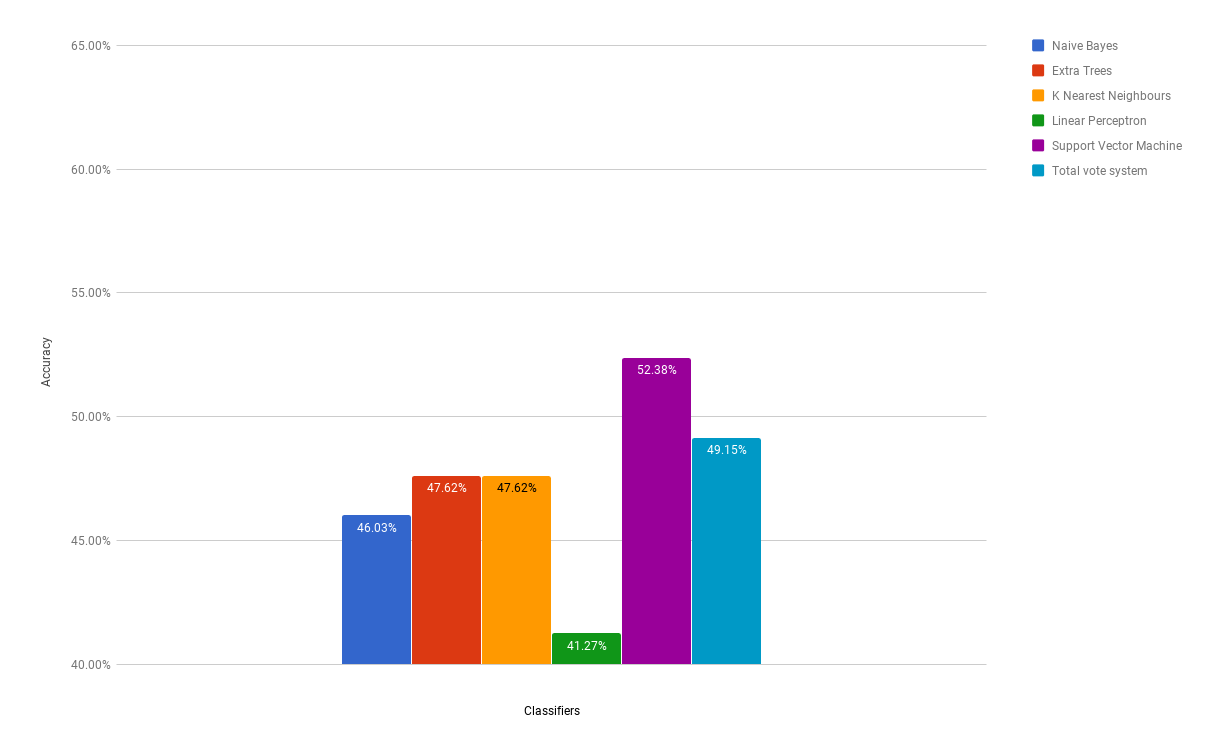
\includegraphics[width=0.80\textwidth]{apple-hour.png}
  \caption{Apple graphs - Hour}
\end{figure}


\subsection{Facebook}

Figure \ref{facebook-hour} shows how the classifiers performed when pedicting the behaviour of the price of shares for Facebook. As can be seen, the classifiers performed worse predicting facebook than they did apple with very low accuracy results across the board. Simialry to the classifications of Apple, it would be better to do a random choice on whether the price is going up or not.

\begin{figure}[h!]
	\label{facebook-hour}
  \centering
  	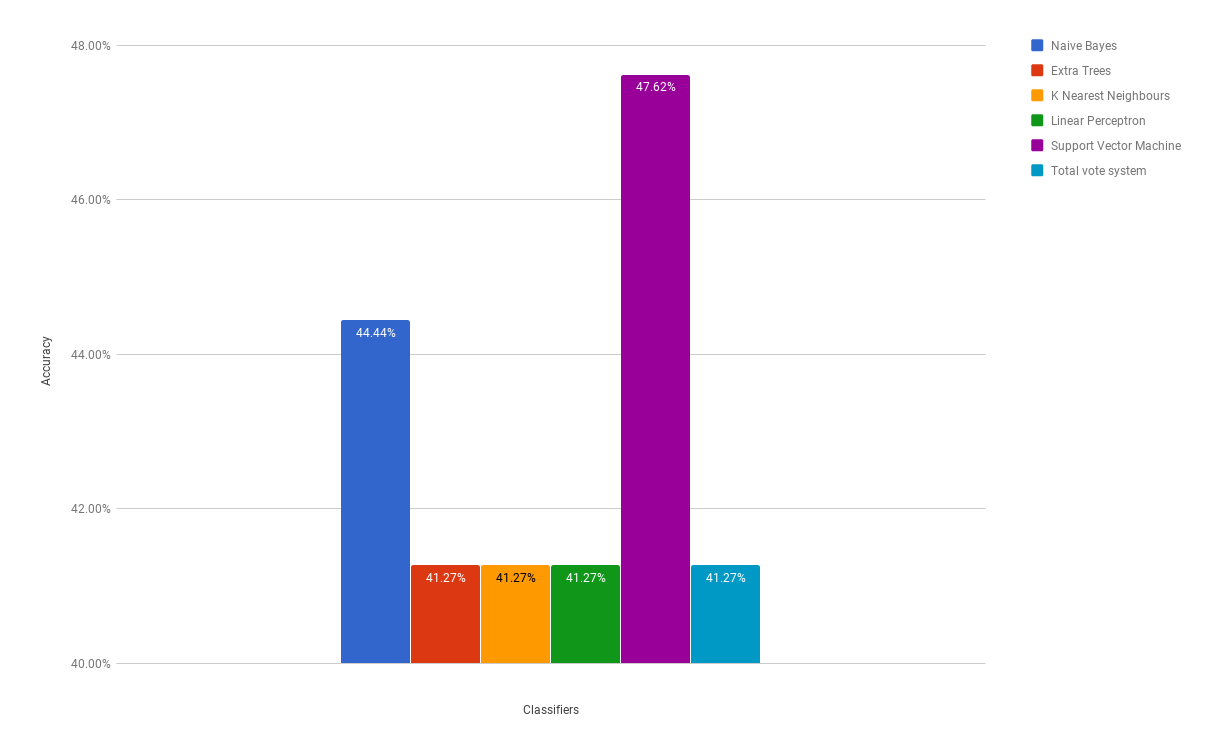
\includegraphics[width=0.80\textwidth]{facebook-hour.png}
  \caption{Facebook graphs - Hour}
\end{figure}

\subsection{Technology}

Compared to the the predictions of Facebook and Apple, judging the whole sector of Technology classifiers performed a lot better. Figure \ref{technology-hour} shows that illustrates that accuracy was above 50\% and would perform better than a random generator. There were very similar results in accuracy between the Naive Bayes, SVM and Extra Trees classifier as well as the total vote peaking at 55.56\%. Linear perceptron performed worst with 52.38\%.


\begin{figure}[h!]
	\label{technology-hour}
  \centering
  	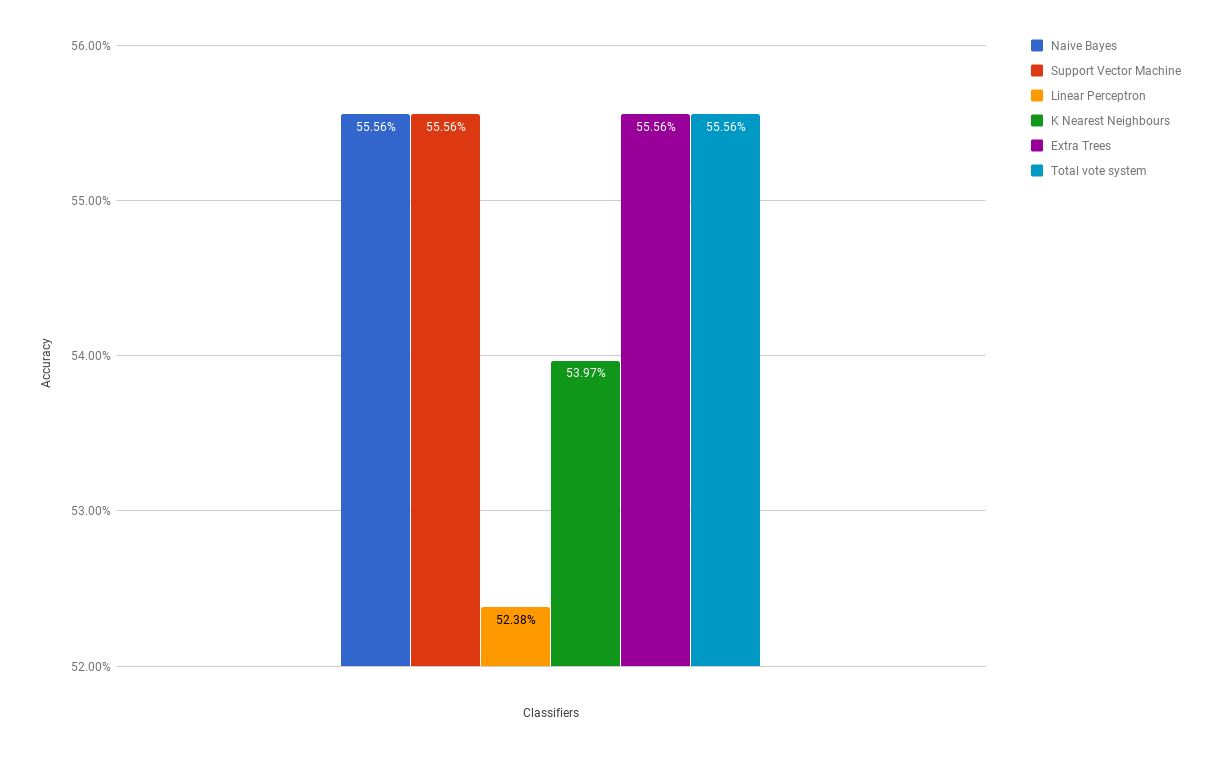
\includegraphics[width=0.80\textwidth]{technology-hour.png}
  \caption{Technology graphs - Hour}
\end{figure}


\subsection{Final comments about hourly predictions}
Reflecting on how well the classfiers predicted sentiment for the hourly behaviour of a share was very poor. The Linear perceptron performed the worst in classifying articles with very poor accuracy in every test. The highest was it's linear classifiers partner the support vector machine. This system is not suited for predicting hourly behaviour and it does not show a correlation.


\section {Day results}

\subsection{Apple}
\begin{figure}[h!]
  \centering
  	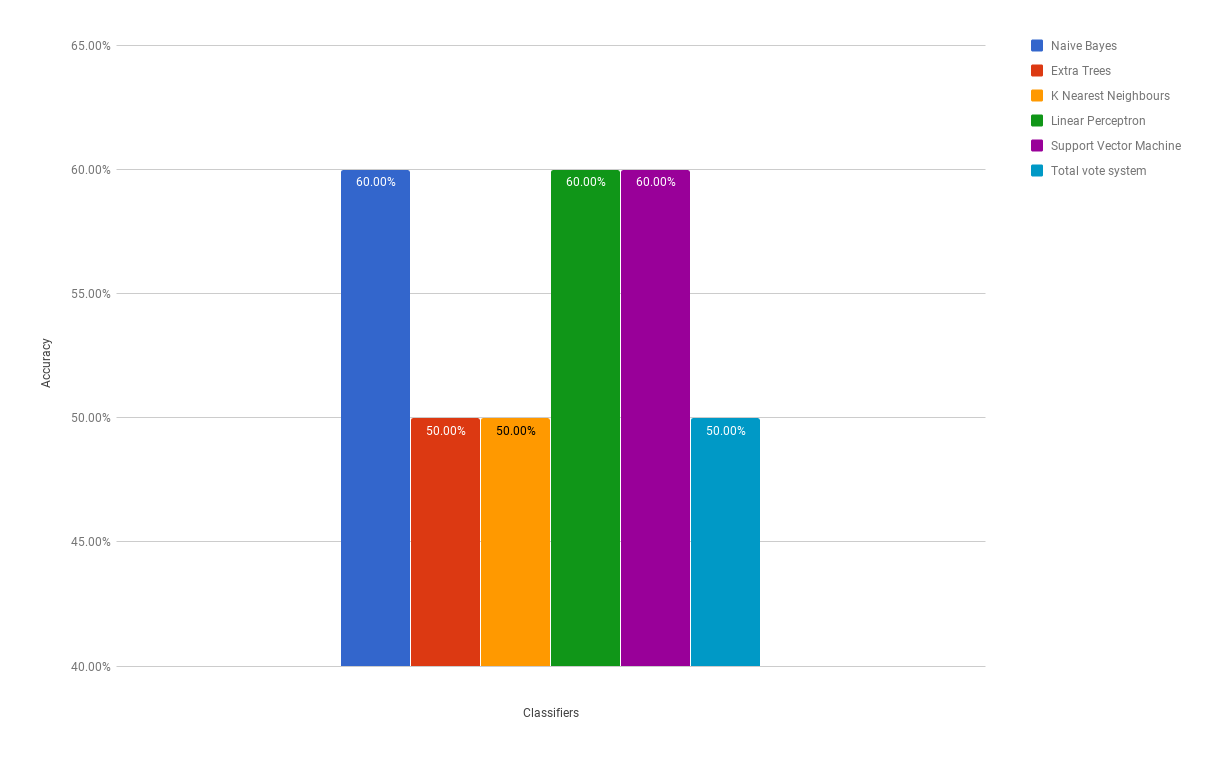
\includegraphics[width=0.70\textwidth]{apple-day.png}
  \caption{Apple graphs - Day}
\end{figure}

\subsection{Facebook}
\begin{figure}[h!]
  \centering
  	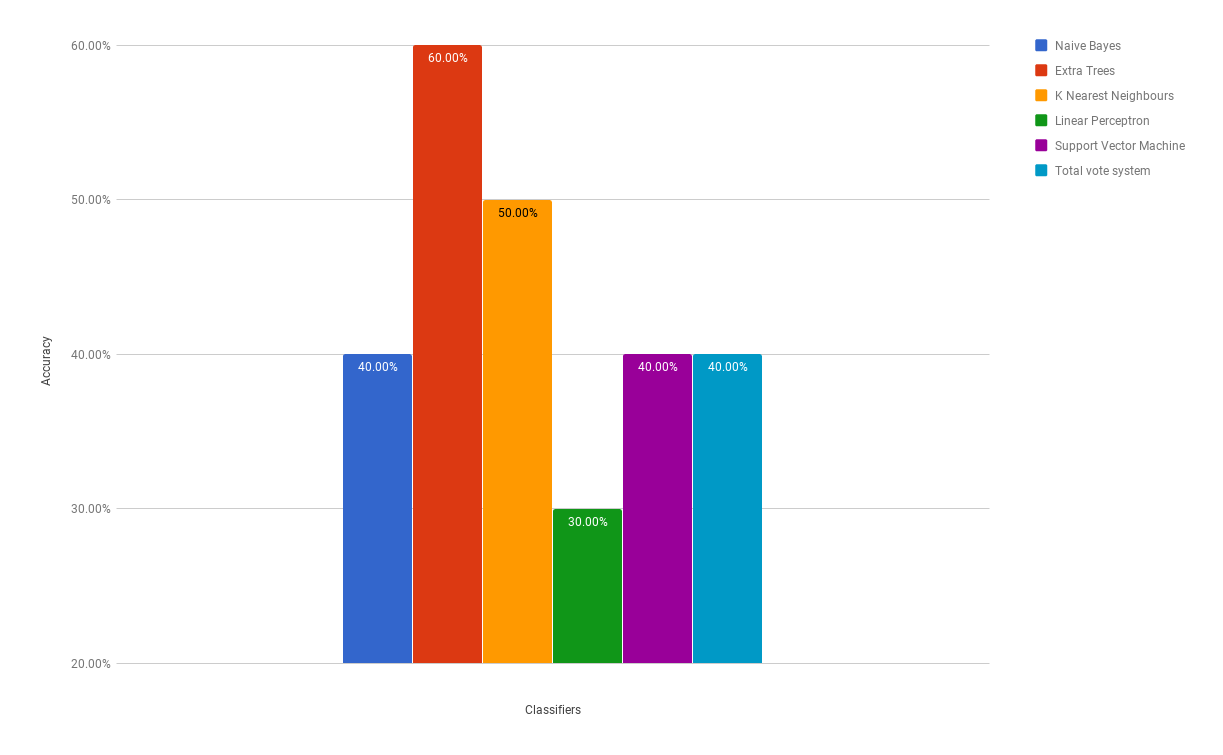
\includegraphics[width=0.70\textwidth]{facebook-day.png}
  \caption{Facebook graphs - Day}
\end{figure}

\subsection{Technology}
\begin{figure}[h!]
  \centering
  	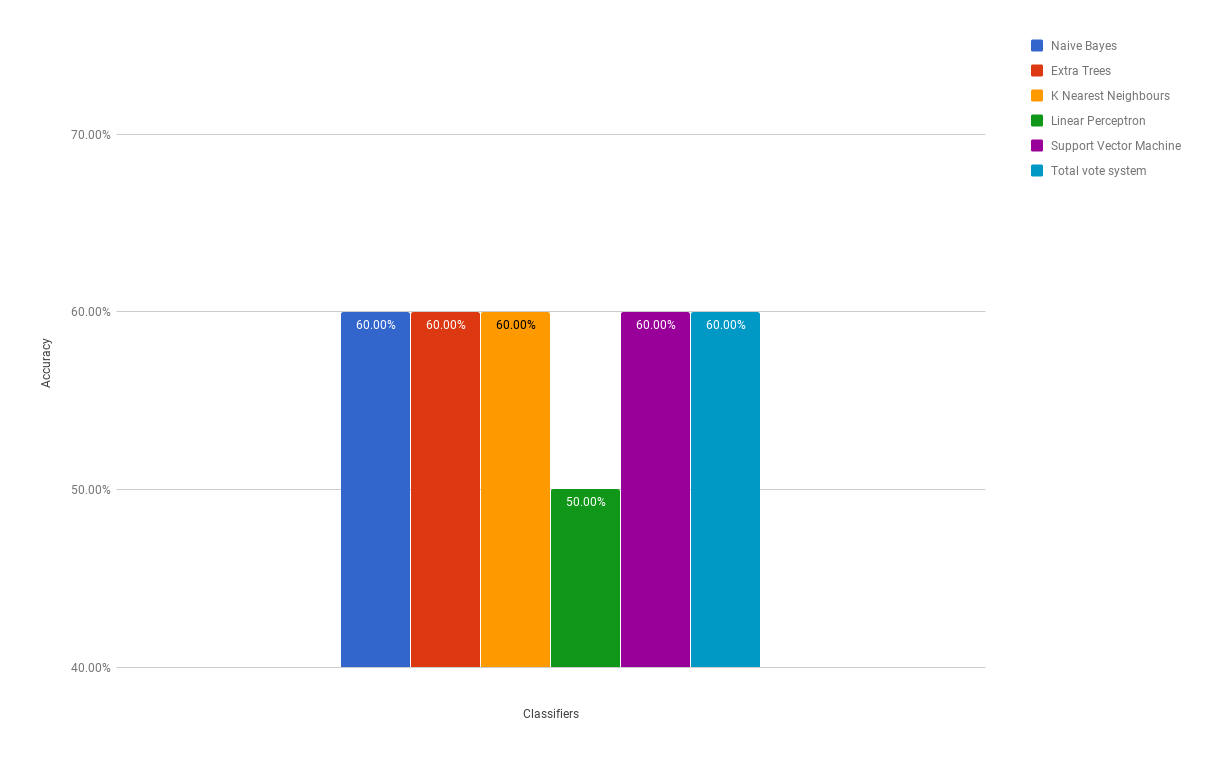
\includegraphics[width=0.70\textwidth]{technology-day.png}
  \caption{Technology graphs - Day}
\end{figure}

\section {Week results}

\subsection{Apple}

\subsection{Facebook}

\subsection{Technology}



%-----------------------------------------------------
% Chapter: Evaluation
%-----------------------------------------------------
\chapter{Evaluation}
\label{chap:evaluation}
\section{Possible Improvements}

%-----------------------------------------------------
% Chapter: Conclusion
%-----------------------------------------------------
\chapter{Conclusion}
\label{chap:conclusion}

\subsection{Further work}



%%%%%%%%%%%%%%%%%%%%%%%%%%%%
% BIBLIOGRAPHY
\clearpage
\phantomsection
\addcontentsline{toc}{chapter}{Bibliography}
\bibliography{bib}
%%%%%%%%%%%%%%%%%%%%%%%%%%%%


%%%%%%%%%%%%%%%%%%%%%%%%%%%%
% START APPENDICES
\appendix
%%%%%%%%%%%%%%%%%%%%%%%%%%%%
\chapter{Designed pipeline}
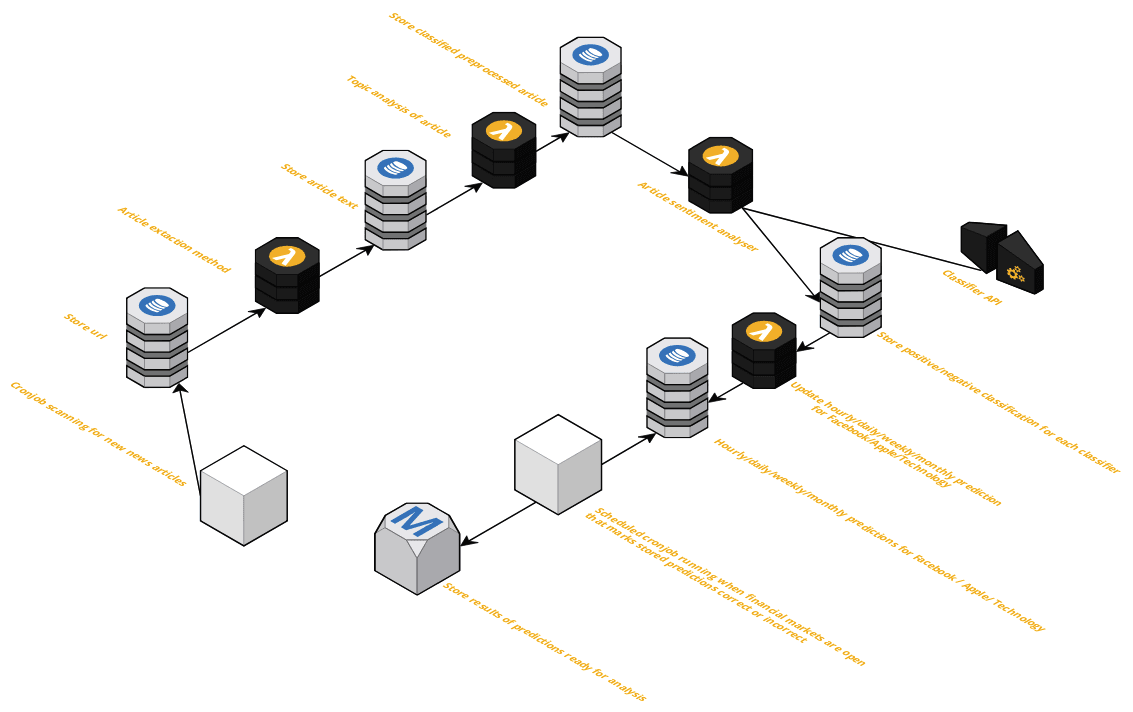
\includegraphics[scale=0.5, angle=90]{pipeline.png}

\begin{table}[h!]
\centering
\caption{TF-IDF using articles content}
\label{tfidf-article-contents}
\begin{tabular}{|l|l|l|}
\hline
                     & Cross-validation accuracy & (+/-)  \\ \hline
Naive Bayes          & 77.65\%                   & 3.12\% \\ \hline
Extra Tree           & 72.16\%                   & 3.60\% \\ \hline
Linear Perceptron    & 76.94\%                   & 4.85\% \\ \hline
SVM                  & 51.21\%                   & 0.05\% \\ \hline
K Nearest Neighbours & 70.29\%                   & 4.14\% \\ \hline
\end{tabular}
\end{table}

\begin{table}[h!]
\centering
\caption{TF-IDF using article summary}
\label{tfidf-article-summary}
\begin{tabular}{|l|l|l|}
\hline
                     & Cross-validation accuracy & (+/-)  \\ \hline
Naive Bayes          & 75.87\%                   & 1.42\% \\ \hline
Extra Tree           & 69.10\%                   & 2.95\% \\ \hline
Linear Perceptron    & 70.45\%                   & 1.96\% \\ \hline
SVM                  & 51.21\%                   & 0.05\% \\ \hline
K Nearest Neighbours & 67.13\%                   & 1.50\% \\ \hline
\end{tabular}
\end{table}

\begin{table}[h!]
\centering
\caption{Count Vectorizer using article contents}
\label{count-article-summary}
\begin{tabular}{|l|l|l|}
\hline
                     & Cross-validation accuracy & (+/-)  \\ \hline
Naive Bayes          & 77.56\%                   & 2.62\% \\ \hline
Extra Tree           & 71.80\%                   & 2.95\% \\ \hline
Linear Perceptron    & 75.46\%                   & 4.45\% \\ \hline
SVM                  & 60.54\%                   & 2.48\% \\ \hline
K Nearest Neighbours & 60.31\%                   & 5.02\% \\ \hline
\end{tabular}
\end{table}


\begin{table}[h!]
\centering
\caption{Count Vectorizer using article summary}
\label{count-article-summary}
\begin{tabular}{|l|l|l|}
\hline
                     & Cross-validation accuracy & (+/-)  \\ \hline
Naive Bayes          & 76.14\%                   & 2.03\% \\ \hline
Extra Tree           & 70.33\%                   & 2.62\% \\ \hline
Linear Perceptron    & 70.06\%                   & 3.29\% \\ \hline
SVM                  & 51.21\%                   & 0.04\% \\ \hline
K Nearest Neighbours & 52.81\%                   & 2.77\% \\ \hline
\end{tabular}
\end{table}


\begin{table}[]
\centering
\caption{Word2Vec using article contents}
\label{w2v-article-content}
\begin{tabular}{|l|l|l|l|}
\hline
                      & Vector Size & Cross-validation accuracy & (+/-)  \\ \hline
Extra Tree            & 50          & 71.06\%                   & 2.95\% \\ \hline
Linear Perceptron     & 50          & 62.13\%                   & 15.03\% \\ \hline
SVM                   & 50          & 75.25\%                   & 2.99\% \\ \hline
K Nearest Neighbours  & 50          & 72.30\%                   & 3.78\% \\ \hline
Extra Tree            & 100         & 70.65\%                   & 2.65\% \\ \hline
Linear Perceptron     & 100         & 61.48\%                   & 4.50\% \\ \hline
SVM                   & 100         & 75.07\%                   & 1.99\% \\ \hline
K Nearest Neighbours  & 100         & 72.02\%                   & 4.51\% \\ \hline
Extra Tree            & 150         & 72.14\%                   & 2.49\% \\ \hline
Linear Perceptron     & 150         & 60.93\%                   & 10.59\% \\ \hline
SVM                   & 150         & 74.93\%                   & 1.63\% \\ \hline
K Neartest Neighbours & 150         & 71.61\%                   & 5.41\% \\ \hline
\end{tabular}
\end{table}

\begin{table}[h!]
\centering
\caption{Word2Vec using article summary}
\label{w2v-article-summary}
\begin{tabular}{|l|l|l|l|}
\hline
                      & Vector Size & Cross-validation accuracy & (+/-)  \\ \hline
Extra Tree            & 50          & 66.60\%                   & 2.55\% \\ \hline
Linear Perceptron     & 50          & 57.76\%                   & 10.60\% \\ \hline
SVM                   & 50          & 72.23\%                   & 2.07\% \\ \hline
K Nearest Neighbours  & 50          & 68.02\%                   & 3.72\% \\ \hline
Extra Tree            & 100         & 67.63\%                   & 3.05\% \\ \hline
Linear Perceptron     & 100         & 58.15\%                   & 12.02\% \\ \hline
SVM                   & 100         & 72.23\%                   & 1.52\% \\ \hline
K Nearest Neighbours  & 100         & 68.25\%                   & 3.11\% \\ \hline
Extra Tree            & 150         & 66.77\%                   & 2.16\% \\ \hline
Linear Perceptron     & 150         & 57.73\%                   & 12.46\% \\ \hline
SVM                   & 150         & 72.25\%                   & 2.24\% \\ \hline
K Neartest Neighbours & 150         & 68.00\%                   & 2.67\% \\ \hline
\end{tabular}
\end{table}

%-----------------------------------------------------
% Appendix: Code
%-----------------------------------------------------
\chapter{Code}
\label{app:code}

\begin{verbatim}
10 PRINT "HELLO WORLD"
\end{verbatim}


%%%%%%%%%%%%%%%%%%%%%%%%%%%%
% END DOCUMENT
\end{document}
%%%%%%%%%%%%%%%%%%%%%%%%%%%%
